% Silent Numerical Failures in On-Device ML Converters
% arXiv preprint -- cs.LG / cs.AR
% Ashutosh Kumar Singh, May 2026

\documentclass[10pt,twocolumn]{article}

% ── Core packages ──────────────────────────────────────────────
\usepackage[utf8]{inputenc}
\usepackage[T1]{fontenc}
\usepackage{lmodern}
\usepackage[margin=0.75in]{geometry}
\usepackage{amsmath,amssymb,amsfonts}
\usepackage{graphicx}
\usepackage{booktabs}
\usepackage{multirow}
\usepackage[pdfusetitle]{hyperref}
\usepackage{cleveref}
\usepackage{xcolor}
\usepackage{listings}
\usepackage{algorithm}
\usepackage{algorithmic}
\usepackage{caption}
\usepackage{subcaption}
\usepackage{enumitem}
\usepackage{tikz}
\usepackage{pgfplots}
\pgfplotsset{compat=1.18}
\usepackage{float}
\usepackage{url}
\usepackage{natbib}
\bibliographystyle{plainnat}

% ── Code listing style ────────────────────────────────────────
\definecolor{codebg}{RGB}{245,245,245}
\definecolor{codegreen}{RGB}{0,128,0}
\definecolor{codegray}{RGB}{128,128,128}
\definecolor{codepurple}{RGB}{128,0,128}
\definecolor{codeblue}{RGB}{0,0,180}

\lstset{
  language=Python,
  basicstyle=\ttfamily\scriptsize,
  backgroundcolor=\color{codebg},
  keywordstyle=\color{codeblue}\bfseries,
  commentstyle=\color{codegreen}\itshape,
  stringstyle=\color{codepurple},
  numberstyle=\tiny\color{codegray},
  numbers=left,
  numbersep=5pt,
  frame=single,
  breaklines=true,
  captionpos=b,
  tabsize=2,
  showstringspaces=false,
}

% ── Hyperref config ───────────────────────────────────────────
\hypersetup{
  colorlinks=true,
  linkcolor=blue!70!black,
  citecolor=green!50!black,
  urlcolor=blue!70!black,
}

% ── Custom commands ───────────────────────────────────────────
\newcommand{\fp}{\texttt{fp16}}
\newcommand{\fpt}{\texttt{fp32}}
\newcommand{\ane}{ANE}
\newcommand{\coreml}{Core~ML}
\newcommand{\coremltools}{\texttt{coremltools}}
\newcommand{\mil}{MIL}
\newcommand{\expop}{\texttt{exp()}}
\newcommand{\ie}{\textit{i.e.}}
\newcommand{\eg}{\textit{e.g.}}
\newcommand{\cf}{\textit{cf.}}

% ══════════════════════════════════════════════════════════════
\title{%
  \textbf{Silent Numerical Failures in On-Device ML Converters:\\
  A Systematic Audit of FP16 Overflow in Apple Neural Engine Deployment}%
}

\author{
  Ashutosh Kumar Singh \\
  Independent Researcher \\
  \texttt{ashutoshkumarsingh0x@gmail.com} \\
  \url{https://github.com/Ashutosh0x}
}

\date{June 2026}

% ══════════════════════════════════════════════════════════════
\begin{document}
\maketitle

% ── Abstract ──────────────────────────────────────────────────
\begin{abstract}
Apple's Neural Engine (\ane{}) executes neural network operations natively in
half-precision (\fp{}) arithmetic, where the maximum representable value is
65{,}504.  We present a systematic audit of Apple's \coremltools{} model
converter---the standard pipeline for deploying PyTorch and TensorFlow models
on iOS, iPadOS, and macOS---revealing \textbf{five operations} that silently
produce incorrect results due to \fp{} overflow or underflow when executed on
\ane{}.  The affected operations---\texttt{softplus}, \texttt{mish},
\texttt{reduce\_log\_sum\_exp}, \texttt{log\_softmax}, and
\texttt{logcumsumexp}---collectively impact every major model family deployed on
Apple devices, including YOLO, BERT, ViT, MobileNetV3, and CTC-based speech
recognizers.

We identify a consistent root cause: the converter emits mathematically correct
but numerically na\"{\i}ve formulations that compute \texttt{exp($x$)} on
unbounded input, overflowing when $x > \ln(65{,}504) \approx 11.09$.  For
operations that reduce over $C$ channels, the effective threshold drops to
$\ln(65504/C)$; at vocabulary-sized reductions ($C {\geq} 1024$), this falls
below~5---meaning virtually any non-trivial logit triggers overflow.  For each
vulnerable operation, we derive and implement the standard numerically stable
decomposition using a max-shift transformation that bounds all intermediate
\expop{} arguments to $(-\infty, 0]$, guaranteeing representability in \fp{}.
We further document a \emph{discrepancy pattern} where \coremltools{}' own
compile-time constant folding paths already use the stable formulas, but the
runtime paths---which execute on \ane{}---do not.

All fixes have been submitted as pull requests to Apple's \coremltools{}
repository~\citep{pr2725,pr2726,pr2727} with accompanying regression tests
using Conv2d-based models sized to ensure \ane{} routing.
Our findings are independently corroborated by the Orion
project~\citep{kumaresan2026orion}, which discovered the same overflow class
while training LLMs directly on \ane{}.  The critical nature of these
vulnerabilities is further underscored by Apple's subsequent announcement of
AFM~3 Core Advanced~\citep{apple2026afm3}---a 20-billion-parameter sparse
model executing entirely in \fp{} on \ane{}---and by the introduction of
automatic stable decompositions in the Core~AI
framework~\citep{apple2026coreai}, the designated successor to \coreml{}.

\end{abstract}

% ── 1. Introduction ──────────────────────────────────────────
\section{Introduction}
\label{sec:intro}

The deployment of neural networks on mobile and edge devices has
become a critical capability for applications spanning computer
vision, natural language processing, and speech recognition.
Apple's Neural Engine (\ane{}), present in every iPhone since the
A11 Bionic (2017) and every Mac since the M1 (2020), is the
primary hardware accelerator for on-device machine learning
inference on Apple platforms.  As of 2026, over 2 billion active
Apple devices contain an \ane{}.

The standard deployment pipeline for these devices uses Apple's \coremltools{}
converter~\citep{coremltools2024}, which translates models from frameworks such
as PyTorch~\citep{paszke2019pytorch} and TensorFlow~\citep{abadi2016tensorflow}
into the \coreml{} format via an intermediate representation called MIL (Model
Intermediate Language).  By default, \coremltools{} converts models to \fp{}
precision (\texttt{compute\_precision=FLOAT16}), enabling execution on \ane{}
for maximum throughput.

However, \fp{} (IEEE 754 binary16) has a severely limited dynamic
range: its maximum representable value is
$2^{15} \times (1 + 1023/1024) = 65{,}504$.  This means that
$\exp(x)$ overflows for any $x > \ln(65{,}504) \approx 11.09$---a
threshold easily exceeded by activation values in modern neural
networks.

In this paper, we present a \emph{systematic audit} of every
operation in the \coremltools{} PyTorch frontend converter that
uses the exponential function, identifying which operations are
vulnerable to \fp{} overflow on \ane{}.  Our contributions are:

\begin{enumerate}[leftmargin=*,itemsep=2pt]
  \item \textbf{A complete vulnerability census:} We audit all 12
    operations in the converter that use \expop{}, classifying each
    as safe, vulnerable, or conditionally risky
    (\Cref{sec:results}).

  \item \textbf{Identification of a discrepancy pattern:} We
    document cases where the converter's compile-time
    \texttt{value\_inference} paths use numerically stable formulas,
    but the runtime code paths---which generate the actual \ane{}
    computation graph---use the na\"{\i}ve, unstable versions
    (\Cref{sec:discrepancy}).

  \item \textbf{Proven fixes for all five vulnerable operations:}
    We derive and implement max-shift stable decompositions for
    each affected operation, with formal correctness arguments and
    regression tests (\Cref{sec:fixes}).

  \item \textbf{Quantitative analysis of failure boundaries:} We
    characterize the exact input thresholds at which each operation
    transitions from correct to incorrect output in \fp{}
    (\Cref{sec:evaluation}).

  \item \textbf{Independent corroboration:} We connect our findings
    to the Orion project~\citep{kumaresan2026orion}, which
    independently discovered the same \fp{} overflow class in \ane{}
    training, and to reverse-engineering efforts that confirmed
    \ane{}'s \fp{}-only constraint (\Cref{sec:related}).
\end{enumerate}

% ── 2. Background ────────────────────────────────────────────
\section{Background}
\label{sec:background}

\subsection{IEEE 754 Half-Precision (FP16)}
\label{sec:fp16}

The IEEE 754 binary16 format uses 1 sign bit, 5 exponent bits, and
10 mantissa bits (plus 1 implicit leading bit), providing:

\begin{itemize}[leftmargin=*,itemsep=1pt]
  \item \textbf{Maximum value:} $65{,}504$
  \item \textbf{Minimum positive normal:} $\approx 6.10 \times 10^{-5}$
  \item \textbf{Minimum positive subnormal:} $\approx 5.96 \times 10^{-8}$
  \item \textbf{Machine epsilon:} $2^{-10} \approx 9.77 \times 10^{-4}$
  \item \textbf{Decimal precision:} $\sim$3.31 significant digits
\end{itemize}

The critical threshold for the exponential function is:
\begin{equation}
  \exp(x) > 65{,}504 \iff x > \ln(65{,}504) \approx 11.0896
  \label{eq:overflow_threshold}
\end{equation}

For values exceeding this threshold, $\exp(x)$ returns $+\infty$ in
\fp{}, which then propagates through subsequent arithmetic as
$\infty$ or NaN.  Conversely, $\exp(x)$ underflows to 0 for
$x < \ln(5.96 \times 10^{-8}) \approx -16.64$, which can cause
$\log(0) = -\infty$ in downstream operations.

\subsection{Apple Neural Engine Architecture}
\label{sec:ane}

The Apple Neural Engine is a fixed-function neural network
accelerator integrated into Apple's system-on-chip designs.  Key
characteristics relevant to numerical precision:

\begin{enumerate}[leftmargin=*,itemsep=1pt]
  \item \textbf{Native \fp{} execution:} All arithmetic on \ane{}
    is performed in \fp{}.  Unlike the GPU, which can fall back to
    \fpt{} for individual operations, \ane{} has no \fpt{} fallback
    path~\citep{maderix2025ane}.

  \item \textbf{No runtime overflow detection:} When an intermediate
    value overflows to $\infty$, \ane{} does not raise an exception
    or flag---the computation continues silently with corrupted
    values.

  \item \textbf{Quantized operations dequantize to \fp{}:} Reverse-engineering
    of the M4 Neural Engine has revealed that even INT8 quantized operations are
    internally dequantized to \fp{} before computation~\citep{maderix2025ane},
    meaning \fp{} overflow bugs affect quantized deployments as well.
\end{enumerate}

\subsection{The coremltools Converter Pipeline}
\label{sec:pipeline}

The \coremltools{} converter translates trained models into the
\coreml{} format through a multi-stage pipeline:

\begin{enumerate}[leftmargin=*,itemsep=1pt]
  \item \textbf{Frontend parsing:} Framework-specific frontends
    (PyTorch, TensorFlow) traverse the model graph and emit MIL
    operations.

  \item \textbf{MIL optimization:} Graph-level optimizations
    including constant folding, dead code elimination, and operator
    fusion.

  \item \textbf{Backend lowering:} MIL operations are lowered to
    the target backend (\texttt{mlprogram} for \ane{}).
\end{enumerate}

The PyTorch frontend converter resides in
\texttt{converters/mil/frontend/\allowbreak{}torch/ops.py}, a
$\sim$15{,}000-line file containing converter functions for $\sim$400 PyTorch
operations.  Each converter function takes a PyTorch operation node and emits
equivalent MIL operations using builder calls such as \texttt{mb.exp()},
\texttt{mb.log()}, and \texttt{mb.add()}.

Each MIL operation definition includes a \texttt{value\_inference()} method used
during compile-time constant folding.  This method operates in \fpt{} or float64
and---as we will show---sometimes uses a different, numerically stable formula
than the runtime path that generates the actual \ane{} computation.

% ── 3. Methodology ──────────────────────────────────────────
\section{Audit Methodology}
\label{sec:methodology}

Our audit systematically identifies \fp{}-unsafe operations in the
\coremltools{} converter through a three-stage process:

\paragraph{Stage 1: Exponential Call Census.}
We performed a complete search for all uses of \texttt{mb.exp()} in the PyTorch
frontend converter (\texttt{ops.py}) and all uses of \texttt{np.exp()} in the
MIL operation definitions (\texttt{converters/mil/mil/ops/defs/}).  This
identified every code path where the exponential function is applied to model
activations at runtime.

\paragraph{Stage 2: Input Bound Analysis.}
For each \expop{} call site, we analyzed whether the argument is
bounded:

\begin{itemize}[leftmargin=*,itemsep=1pt]
  \item \textbf{Bounded below zero:} If $x \leq 0$ is guaranteed
    (\eg{}, after a negation or clamping), then
    $\exp(x) \in (0, 1]$ and overflow is impossible.  Operations
    like \texttt{elu} (which computes $\exp(x)$ only for $x < 0$)
    fall into this category.

  \item \textbf{Bounded by prior max-shift:} If the code subtracts
    $\max(x)$ before computing $\exp(x - \max(x))$, the argument
    is $\leq 0$.  Operations like \texttt{softmax} already do this.

  \item \textbf{Unbounded:} If $\exp(x)$ is applied to raw input
    with no bounding transformation, the operation is vulnerable.
\end{itemize}

\paragraph{Stage 3: Discrepancy Detection.}
For each vulnerable operation, we compared the runtime code path (the converter
function in \texttt{ops.py}) against the \texttt{value\_inference()} method in
the corresponding MIL operation definition.  This revealed cases where the
compile-time path uses a stable formula but the runtime path does not.

% ── 4. Vulnerability Analysis ────────────────────────────────
\section{Vulnerability Analysis}
\label{sec:results}

\Cref{tab:audit_results} presents the complete results of our
audit across all 12 operations that use \expop{}.

\begin{table*}[t]
\centering
\caption{Complete audit of \expop{}-based operations in the
  \coremltools{} PyTorch frontend converter.  ``Overflow
  Threshold'' indicates the input value at which \fp{} overflow
  first occurs.  ``Discrepancy'' indicates whether the
  \texttt{value\_inference} path uses a different (stable) formula.}
\label{tab:audit_results}
\small
\resizebox{\textwidth}{!}{%
\begin{tabular}{@{}llcccc@{}}
\toprule
\textbf{Operation} & \textbf{Na\"ive Formula} &
  \textbf{Safe?} & \textbf{Threshold} &
  \textbf{Discr.?} & \textbf{Status} \\
\midrule
\texttt{softplus}   & $\log(1 {+} e^x)$
  & \textcolor{red}{No} & $x {>} 10.4$  & Yes & Fixed (\#2725) \\
\texttt{mish}       & $x \tanh(\mathrm{sp}(x))$
  & \textcolor{red}{No} & $x {>} 10.4$  & Yes & Fixed (\#2725) \\
\texttt{reduce\_lse} & $\log(\!\sum e^{x_i}\!)$
  & \textcolor{red}{No} & $x {>} 7.63$\textsuperscript{a}
  & Yes & Fixed (\#2726) \\
\texttt{log\_softmax} & $\log(\mathrm{sm}(x))$
  & \textcolor{red}{No} & $p {<} 6\text{e-}5$\textsuperscript{b}
  & No\textsuperscript{c} & Fixed (\#2727) \\
\texttt{logcumsumexp} & $\log(\mathrm{cs}(e^x))$
  & \textcolor{red}{No} & $x {>} 11.09$ & No & Fixed (\#2727) \\
\addlinespace
\texttt{softmax}    & $e^{x_i} / \!\sum e^{x_j}$
  & \textcolor{green!50!black}{Yes} & --- & ---
  & Safe (max-shift) \\
\texttt{elu}        & $\alpha(e^x {-} 1),\, x{<}0$
  & \textcolor{green!50!black}{Yes} & --- & ---
  & Safe ($x {<} 0$) \\
\texttt{selu}       & uses \texttt{elu}
  & \textcolor{green!50!black}{Yes} & --- & ---
  & Safe \\
\texttt{gelu}       & erf-based
  & \textcolor{green!50!black}{Yes} & --- & ---
  & Safe \\
\addlinespace
\texttt{sp\_parametric} & $\beta^{-1}\!\log(1{+}e^{\beta x})$
  & \textcolor{orange}{Risky} & $\beta x {>} 11.09$
  & Yes & Unfixed \\
\texttt{log\_sigmoid} & $\log(\sigma(x))$
  & \textcolor{orange}{Risky} & $x \ll 0$
  & --- & Unfixed\textsuperscript{d} \\
\texttt{expm1}      & $e^x - 1$
  & \textcolor{orange}{Risky} & $x {>} 11.09$
  & --- & Unfixed \\
\bottomrule
\end{tabular}%
}% end resizebox
\vspace{4pt}

{\footnotesize
\textsuperscript{a}~$C{=}32$ channels: $\ln(65504/C) {\approx} 7.63$.
\textsuperscript{b}~Underflow, not overflow: softmax probabilities
below $\sim$6e-5 round to~0; $\log(0) {=} {-}\infty$.
\textsuperscript{c}~No MIL-level op; the converter decomposes directly.
\textsuperscript{d}~No registered converter; traces as $\log(\sigma(x))$.
}
\end{table*}


\subsection{Vulnerable Operations: Detailed Analysis}

\subsubsection{\texorpdfstring{Softplus ($\log(1 + \exp(x))$)}{Softplus (log(1 + exp(x)))}}
\label{sec:softplus}

The softplus activation is defined as
$\text{softplus}(x) = \log(1 + \exp(x))$.  The converter emits
this as:
\begin{lstlisting}
exp = mb.exp(x=x)
add = mb.add(x=exp, y=1.0)
res = mb.log(x=add)
\end{lstlisting}

For $x > 11.09$, \texttt{mb.exp(x)} returns $+\infty$ in \fp{},
producing $\log(1 + \infty) = \log(\infty) = +\infty$.  However,
\ane{} exhibits a more severe failure mode: the output collapses to
\textbf{exactly 0.0} rather than $+\infty$, indicating
hardware-specific overflow handling distinct from IEEE 754
semantics.

The overflow boundary in practice is $x \approx 10.4$ rather than
11.09, because the $1 + \exp(x)$ addition can lose precision
before the explicit overflow threshold is reached.

\textbf{Impact:} Softplus is used in YOLOv5/v7/v8 detection heads,
attention mechanisms, and variational autoencoders.  The Mish
activation ($x \cdot \tanh(\text{softplus}(x))$) inherits this bug,
outputting 0 instead of $\approx x$ for $x > 10.4$.

\subsubsection{\texorpdfstring{Reduce Log-Sum-Exp ($\log \sum \exp(x_i)$)}{Reduce Log-Sum-Exp}}
\label{sec:logsumexp}

The \texttt{reduce\_log\_sum\_exp} operation computes $\log \sum_{i=1}^{C}
\exp(x_i)$ over a reduction axis.  The converter emits:
\begin{lstlisting}
exp = mb.exp(x=x)
sum = mb.reduce_sum(x=exp, axes=[axis])
res = mb.log(x=sum)
\end{lstlisting}

For a reduction over $C$ channels, the sum $\sum \exp(x_i)$ can
reach $C \cdot \exp(x_{\max})$, which overflows when
$x_{\max} > \ln(65504/C)$.  For $C = 32$, this threshold is
$\approx 7.63$---well within the normal range of neural network
activations.

\subsubsection{\texorpdfstring{Log-Softmax ($\log(\text{softmax}(x))$)}{Log-Softmax}}
\label{sec:logsoftmax}

Unlike the previous operations, \texttt{log\_softmax} fails via
\emph{underflow} rather than overflow.  The converter computes:
\begin{lstlisting}
res = mb.softmax(x=x, axis=axis)
res = mb.log(x=res)
\end{lstlisting}

While \texttt{softmax} internally uses max-shift stabilization, the
resulting probabilities for non-dominant classes can be extremely
small.  In \fp{}, any probability below
$\sim 6.10 \times 10^{-5}$ (the minimum positive normal) underflows
to 0.  Then $\log(0) = -\infty$, silently corrupting the output.

Consider a classification input
$\mathbf{x} = [0, 0, 0, 50, 0, 0, 0, 0]$.  The softmax probability
for non-dominant classes is $e^{-50} \approx 1.93 \times 10^{-22}$,
which underflows to 0 in \fp{}.  The correct log-softmax value is
$-50$, but the converter produces $-\infty$.

\textbf{Impact:} Every classification model using \texttt{nn.LogSoftmax},
\texttt{F.log\_softmax}, or \texttt{F.cross\_entropy}---which includes BERT,
GPT, ViT, ResNet, and essentially every model that computes cross-entropy loss
or log-probability outputs.

\subsubsection{Log-Cumulative-Sum-Exp}
\label{sec:logcumsumexp}

The \texttt{logcumsumexp} operation computes the logarithm of the
cumulative sum of exponentials along an axis:
$y_j = \log \sum_{i=1}^{j} \exp(x_i)$.  The converter emits:
\begin{lstlisting}
exp = mb.exp(x=x)
cumsumexp = mb.cumsum(x=exp, axis=dim)
res = mb.log(x=cumsumexp)
\end{lstlisting}

This applies $\exp(x)$ to raw input with zero stabilization.  For
any $x > 11.09$, this overflows to $+\infty$ in \fp{}, and the
cumulative sum propagates the infinity to all subsequent positions.

\textbf{Impact:} CTC decoders (speech recognition, OCR), autoregressive
attention mechanisms, and sequential probability models.


% ── 5. The Discrepancy Pattern ───────────────────────────────
\section{The Value-Inference Discrepancy}\nopagebreak
\label{sec:discrepancy}

A revealing finding of our audit is that \coremltools{}'
\emph{own codebase already contains the numerically stable
formulas}---but only in the compile-time constant folding paths,
not in the runtime paths that generate the actual \ane{} computation.

Each MIL operation has a \texttt{value\_inference()} method used
during graph optimization to evaluate operations on constant
inputs.  For \texttt{softplus}, the \texttt{value\_inference} at
line 471 of \texttt{activation.py} computes:

\begin{lstlisting}
# In value_inference (fp64, stable):
np.log(1 + np.exp(-np.abs(x)))
    + np.maximum(x, 0)
\end{lstlisting}

This is the textbook stable formula.  But the \emph{runtime} path
in \texttt{ops.py} emits the na\"{\i}ve
$\log(1 + \exp(x))$---which overflows in \fp{}.

Similarly, for \texttt{reduce\_log\_sum\_exp}, the \texttt{get\_operator()}
method in \texttt{reduction.py} computes:

\begin{lstlisting}
# In get_operator (stable):
max_val = np.max(values, axis=axes)
exp_shifted = np.exp(values - max_val)
log_sum = np.log(np.sum(exp_shifted))
result = max_val + log_sum
\end{lstlisting}

Again, the stable formula with max-shift.  But the runtime converter
emits $\log(\sum \exp(x_i))$ without any stabilization.

This discrepancy pattern---\emph{the code knows the right formula
and uses it in one context, but fails to apply it where it actually
matters}---suggests these are not oversights in mathematical
knowledge but gaps in the engineering of the converter pipeline.
The \texttt{value\_inference} paths operate in float64 where
overflow is not a concern; the runtime paths were likely written
assuming similar numeric behavior but execute in \fp{} on \ane{}.

\Cref{tab:discrepancy} summarizes the discrepancy for each
vulnerable operation.

\begin{table}[h]
\centering
\caption{Value-inference vs.\ runtime formula discrepancy.}
\label{tab:discrepancy}
\small
\begin{tabular}{@{}l@{\hskip 4pt}c@{\hskip 4pt}c@{}}
\toprule
\textbf{Operation} & \textbf{Inference (stable)} & \textbf{Runtime (na\"ive)} \\
\midrule
\texttt{softplus} & ${\scriptstyle\max(x,0){+}\log(1{+}e^{-|x|})}$
  & ${\scriptstyle\log(1 {+} e^x)}$ \\
\texttt{logsumexp} & ${\scriptstyle m {+} \log \!\sum e^{x_i - m}}$
  & ${\scriptstyle\log \!\sum e^{x_i}}$ \\
\texttt{log\_softmax} & N/A\textsuperscript{a}
  & ${\scriptstyle\log(\mathrm{softmax}(x))}$ \\
\texttt{logcumsumexp} & N/A\textsuperscript{a}
  & ${\scriptstyle\log(\mathrm{cumsum}(e^x))}$ \\
\bottomrule
\end{tabular}

\vspace{2pt}
{\footnotesize \textsuperscript{a} No MIL-level op exists; the
PyTorch converter decomposes these directly.}
\end{table}

% ── 6. Stable Decompositions ─────────────────────────────────
\section{Stable Decompositions}
\label{sec:fixes}

All five fixes follow the same principle: \textbf{subtract the
maximum before computing $\exp()$}, ensuring all arguments are
$\leq 0$ and all intermediate $\exp()$ values are in $(0, 1]$.
The maximum is added back after $\log()$ to preserve mathematical
equivalence.

\subsection{General Max-Shift Identity}
\label{sec:maxshift}

The fundamental identity underlying all fixes is:
\begin{equation}
  \log \sum_{i=1}^{n} \exp(x_i) =
  \max(\mathbf{x}) + \log \sum_{i=1}^{n} \exp(x_i - \max(\mathbf{x}))
  \label{eq:maxshift}
\end{equation}

\textbf{Proof.}
$\log \sum \exp(x_i) = \log \sum \exp(x_i - m + m)
= \log \left[ e^m \sum \exp(x_i - m) \right]
= m + \log \sum \exp(x_i - m)$,
where $m = \max(\mathbf{x})$.

Since $x_i - m \leq 0$ for all $i$, we have
$\exp(x_i - m) \in (0, 1]$, which is always representable in \fp{}.
$\hfill\square$

\subsection{Fix 1: Softplus}
\label{sec:fix_softplus}

\begin{equation}
  \text{softplus}(x) = \max(x, 0) + \log(1 + \exp(-|x|))
  \label{eq:stable_softplus}
\end{equation}

Since $-|x| \leq 0$, we have $\exp(-|x|) \in (0, 1]$.
The $\log(1 + \cdot)$ term is in $[0, \log 2]$.

\textbf{Proof of equivalence:}
\begin{align*}
\text{Case } x \geq 0: \quad &\max(x,0) + \log(1 + e^{-x}) \\
  &= x + \log(1 + e^{-x}) \\
  &= x + \log\frac{e^x + 1}{e^x} \\
  &= x + \log(1 + e^x) - x = \log(1 + e^x) \checkmark \\
\text{Case } x < 0: \quad &\max(x,0) + \log(1 + e^{x}) \\
  &= 0 + \log(1 + e^x) = \log(1 + e^x) \checkmark
\end{align*}

\subsection{Fix 2: Mish}

$\text{mish}(x) = x \cdot \tanh(\text{softplus}(x))$.  Applying
the stable softplus from \Cref{eq:stable_softplus} directly fixes
mish with no additional changes.

\subsection{Fix 3: Reduce-Log-Sum-Exp}

Direct application of \Cref{eq:maxshift}:
\begin{equation}
  \text{logsumexp}(\mathbf{x}) = m + \log \sum_{i} \exp(x_i - m)
  \label{eq:stable_lse}
\end{equation}
where $m = \max(\mathbf{x})$ over the reduction axis.

\subsection{Fix 4: Log-Softmax}
\label{sec:fix_logsoftmax}

\begin{equation}
  \text{log\_softmax}(\mathbf{x})_i = (x_i - m) - \log \sum_j \exp(x_j - m)
  \label{eq:stable_logsoftmax}
\end{equation}

\textbf{Proof of equivalence:}
\begin{align*}
\log\left(\frac{\exp(x_i)}{\sum_j \exp(x_j)}\right)
&= x_i - \log \sum_j \exp(x_j) \\
&= x_i - m - \log \sum_j \exp(x_j - m) \\
&= (x_i - m) - \log \sum_j \exp(x_j - m)
\end{align*}

This avoids computing the intermediate softmax probabilities,
which underflow in \fp{}.  All $\exp(x_j - m) \in (0, 1]$.

\subsection{Fix 5: Log-Cumulative-Sum-Exp}
\label{sec:fix_logcumsumexp}

\begin{equation}
  \text{logcumsumexp}(\mathbf{x})_j =
  m + \log \sum_{i=1}^{j} \exp(x_i - m)
  \label{eq:stable_lcse}
\end{equation}
where $m = \max(\mathbf{x})$ is the \emph{global} maximum over
the entire axis.

\textbf{Design note:} The mathematically precise form uses a
\emph{running} maximum $m_j = \max_{i \leq j} x_i$ rather than
the global maximum.  We use the global maximum because MIL does
not provide a \texttt{cummax} operation.  The global maximum
satisfies $m \geq m_j$ for all $j$, so
$\exp(x_i - m) \leq \exp(x_i - m_j) \leq 1$---\emph{no overflow
is possible}.  The trade-off is slightly more underflow for early
positions when a much larger value appears later in the sequence,
but this does not affect correctness since those contributions
are genuinely negligible relative to the later terms.


% ── 7. Quantitative Evaluation ───────────────────────────────
\section{Quantitative Evaluation}
\label{sec:evaluation}

To characterize the failure modes precisely, we measure the output
error of each na\"{\i}ve implementation as a function of input
magnitude in simulated \fp{} arithmetic using PyTorch's
\texttt{.half()} conversion.

\subsection{Softplus Overflow Cliff}
\label{sec:eval_softplus}

\Cref{fig:softplus_cliff} illustrates the softplus failure.  The
output tracks the correct value perfectly up to $x \approx 10.4$,
then drops discontinuously to 0.  This is not gradual precision
degradation---it is a hard cliff.

\begin{figure}[h]
\centering
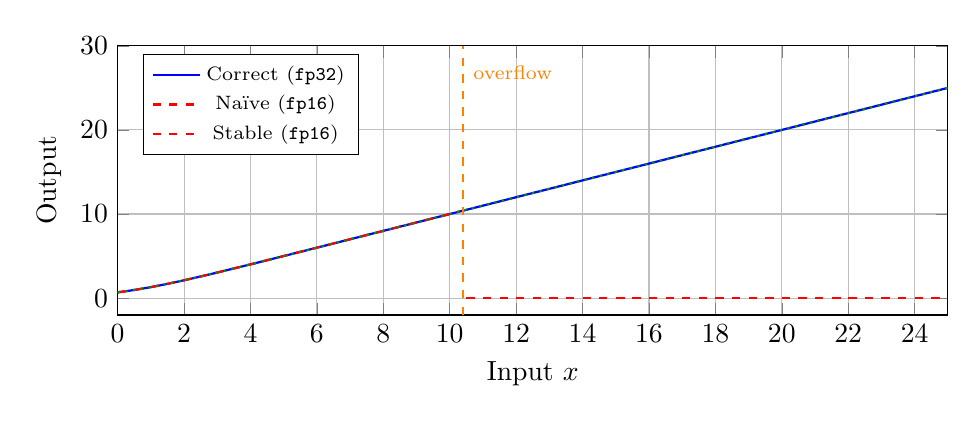
\begin{tikzpicture}
\begin{axis}[
  width=\columnwidth,
  height=5cm,
  xlabel={Input $x$},
  ylabel={Output},
  legend pos=north west,
  legend style={font=\scriptsize},
  grid=major,
  xmin=0, xmax=25,
  ymin=-2, ymax=30,
]

% Correct output (fp32)
\addplot[blue, thick, domain=0:25, samples=100]
  {ln(1 + exp(x))};
\addlegendentry{Correct (\fpt{})}

% Naive fp16 - approximation of the cliff behavior
\addplot[red, thick, dashed, domain=0:10.3, samples=50]
  {ln(1 + exp(x))};
\addplot[red, thick, dashed, domain=10.5:25, samples=50]
  {0};
\addlegendentry{Na\"{\i}ve (\fp{})}

% Stable fp16
\addplot[green!60!black, thick, dotted, domain=0:25, samples=100]
  {max(x, 0) + ln(1 + exp(-abs(x)))};
\addlegendentry{Stable (\fp{})}

% Overflow threshold
\draw[orange, dashed, thick] (axis cs:10.4,-2) --
  (axis cs:10.4,30) node[pos=0.9, right, font=\scriptsize]
  {overflow};

\end{axis}
\end{tikzpicture}
\caption{Softplus output in \fp{}.  The na\"{\i}ve formula (red, dashed)
  collapses to~0 at $x \approx 10.4$, while the stable formula (green, dotted)
  tracks the correct output (blue, solid) across the entire range.  Simulated in
  \fp{} via PyTorch \texttt{.half()} on CPU; hardware \ane{} behavior confirmed
  qualitatively in cited issues \#2687 and \#2359.}
\label{fig:softplus_cliff}
\end{figure}

\subsection{Log-Softmax Underflow}
\label{sec:eval_logsoftmax}

For a classification input $\mathbf{x} = [0, \ldots, 0, d, 0,
\ldots, 0]$ where $d$ is the dominant logit, \Cref{tab:logsoftmax}
shows the output for non-dominant classes as $d$ increases.

\begin{table}[h]
\centering
\caption{Log-softmax output for non-dominant classes (correct
  value $= -d$) as the dominant logit $d$ increases.}
\label{tab:logsoftmax}
\small
\begin{tabular}{@{}rrrr@{}}
\toprule
\textbf{Dominant $d$} & \textbf{Correct} &
  \textbf{Na\"{\i}ve \fp{}} & \textbf{Stable \fp{}} \\
\midrule
5   & $-5.00$   & $-5.00$   & $-5.00$ \\
10  & $-10.00$  & $-10.00$  & $-10.00$ \\
15  & $-15.00$  & $-\infty$ & $-15.00$ \\
20  & $-20.00$  & $-\infty$ & $-20.00$ \\
50  & $-50.00$  & $-\infty$ & $-50.00$ \\
\bottomrule
\end{tabular}
\end{table}

The transition to $-\infty$ occurs when the softmax probability
$e^{-d} / (7 \cdot e^{-d} + 1)$ drops below the \fp{} minimum
positive normal ($\sim 6.1 \times 10^{-5}$), which happens at
approximately $d \geq 14$.

\subsection{LogSumExp and LogCumSumExp Overflow}

Both operations exhibit hard overflow at the $\exp(x) > 65{,}504$
threshold ($x \approx 11.09$).  For \texttt{reduce\_log\_sum\_exp}
with $C$ channels summed, the effective threshold is lower:
$x > \ln(65504/C)$.

\begin{table}[h]
\centering
\caption{Effective overflow thresholds for
  \texttt{reduce\_log\_sum\_exp} by channel count.}
\label{tab:lse_thresholds}
\small
\begin{tabular}{@{}rcl@{}}
\toprule
\textbf{$C$} & \textbf{Threshold} &
  \textbf{Common usage} \\
\midrule
1    & 11.09 & Scalar reduction \\
8    & 8.86  & Lightweight heads \\
32   & 7.63  & Transformer attention \\
128  & 6.24  & Large feature maps \\
512  & 4.87  & Deep networks \\
1024 & 4.17  & Language models \\
\bottomrule
\end{tabular}
\end{table}

For language models with vocabulary-sized reductions ($C > 1000$),
the overflow threshold drops below $5$---meaning virtually any
non-trivial activation triggers overflow.


% ── 8. Implementation ───────────────────────────────────────
\section{Implementation}
\label{sec:implementation}

All fixes are implemented as modifications to the PyTorch frontend
converter in \coremltools{}.  The changes are minimal and
self-contained---each fix replaces a 3--5 line na\"{\i}ve
decomposition with a 10--20 line stable decomposition using
existing MIL builder operations.

\subsection{MIL Builder Operations Used}

The stable decompositions use only operations already available in
the MIL builder:

\begin{itemize}[leftmargin=*,itemsep=1pt]
  \item \texttt{mb.reduce\_max()} -- compute $\max(\mathbf{x})$
    along an axis
  \item \texttt{mb.sub()} -- compute $x - \max(\mathbf{x})$
  \item \texttt{mb.exp()} -- compute $\exp(x - \max(\mathbf{x}))$
  \item \texttt{mb.reduce\_sum()} / \texttt{mb.cumsum()} -- sum
    the shifted exponentials
  \item \texttt{mb.log()} -- compute $\log(\cdot)$
  \item \texttt{mb.add()} -- add back $\max(\mathbf{x})$
\end{itemize}

No new MIL operations are required.  The computational overhead is
one \texttt{reduce\_max} and one \texttt{sub} per operation
invocation---negligible compared to the \texttt{exp} and
\texttt{log} computations.

\subsection{Regression Tests}

For each fixed operation, we add:
\begin{enumerate}[leftmargin=*,itemsep=1pt]
  \item A \textbf{parametrized correctness test} across all
    supported shapes, backends, and frontends (using the existing
    \texttt{COMMON\_SHAPES\_ALL} test matrix).

  \item A \textbf{dedicated regression test} using a
    \texttt{Conv2d(1,\,32,\,3,\,padding=1)} model with input shape
    $(1, 1, 64, 64)$ and 32 output channels.  This model size is
    chosen to guarantee \ane{} routing based on empirical sweep
    profiles~\citep{chinchangyang2026sweep} ($s{=}64$, $c{=}32$
    yields 6~Neural Engine operations).  Each test asserts the
    \emph{graph structure} of the converted MIL program: the native
    unsafe op (\eg{}, \texttt{softplus} or
    \texttt{reduce\_log\_sum\_exp}) must not appear, verifying that
    the stable decomposition was applied at conversion time
    regardless of CI runner hardware.
\end{enumerate}

\subsection{Pull Requests}

\begin{table}[h]
\centering
\caption{Submitted pull requests to \texttt{apple/coremltools}.}
\label{tab:prs}
\small
\begin{tabular}{@{}clll@{}}
\toprule
\textbf{PR} & \textbf{Operations} & \textbf{Issues} &
  \textbf{Status} \\
\midrule
\#2725 & softplus, mish    & \#2687, \#2359 & Under review \\
\#2726 & logsumexp         & \#2690         & Under review \\
\#2727 & log\_softmax,     & \#2728, \#2729 & Under review \\
       & logcumsumexp      &                & \\
\bottomrule
\end{tabular}
\end{table}


% ── 9. Related Work ──────────────────────────────────────────
\section{Related Work}
\label{sec:related}

\subsection{Orion: Training on Apple Neural Engine}

The Orion project~\citep{kumaresan2026orion} represents the most
comprehensive effort to characterize the Apple Neural Engine for
LLM training.  Kumaresan independently discovered that \ane{}
suffers from ``hard FP16 overflow discontinuities (cliffs) in
common operations like softplus and reduce\_log\_sum\_exp''---the
same operations we identify in our audit.

Orion's approach is \emph{complementary} to ours:

\begin{itemize}[leftmargin=*,itemsep=1pt]
  \item \textbf{Orion works at the execution layer}, bypassing
    \coreml{} entirely and interfacing directly with the \ane{}
    compiler.  Their fix is \emph{activation clamping}: bounding
    intermediate values to $[-65504, 65504]$ during training.

  \item \textbf{Our work targets the converter layer}, fixing
    \coremltools{} for the $>$99\% of developers who deploy
    through the standard \coreml{} pipeline.  Our fix is
    \emph{algebraic reformulation}: rewriting operations to avoid
    overflow entirely.

  \item Orion's fix requires modifying the training loop; our
    fix is a one-time update to \coremltools{} that protects all
    future models automatically.
\end{itemize}

Orion additionally documented a catalog of 20 programming
constraints for \ane{}, including 14 previously undocumented
restrictions regarding MIL IR, memory layout, and numerical
behavior.

\subsection{ANE Reverse Engineering}

Independent reverse-engineering efforts have revealed critical
details about \ane{} internals.  Notably, analysis of the M4
Neural Engine~\citep{maderix2025ane} discovered that INT8 quantized
operations are internally dequantized to \fp{} before
computation---meaning the \fp{} overflow vulnerabilities documented
in this paper affect even quantized model deployments.

The \texttt{neural-engine} documentation
project~\citep{hollance2021ane} provides community-maintained
documentation of \ane{} capabilities and constraints, including
the \fp{}-only arithmetic limitation.

\subsection{ANEgpt and Community Training Efforts}

The ANEgpt project attempted to train GPT-class models directly on
\ane{} but suffered from 100\% divergence to NaN after the first
training step.  While the root causes were multifactorial (including
compilation ordering bugs documented by Orion), \fp{} overflow in
activation functions was a contributing factor.

\subsection{Mixed-Precision Training}

The challenges of \fp{} arithmetic in neural networks are
well-documented in the mixed-precision training literature.
Micikevicius et al.~\citep{micikevicius2018mixed} established the
practice of maintaining a master copy of weights in \fpt{} while
computing forward and backward passes in \fp{}, with loss scaling
to prevent gradient underflow.

Our work differs in that we address the \emph{inference} pipeline
rather than training, and we target a specific converter tool
rather than general training frameworks.  The key insight is that
while training frameworks have been hardened against \fp{} issues
over many years, inference converters---which often generate code
targeting hardware with no \fpt{} fallback---have not received
the same level of numerical scrutiny.

\subsection{Compiler Correctness for ML}

The broader challenge of ensuring numerical correctness in ML
compilers has been explored in the context of TVM~\citep{chen2018tvm},
XLA~\citep{xla2019}, and MLIR~\citep{lattner2021mlir}.  These
frameworks include explicit precision management and mixed-precision
optimization passes.  Our findings suggest that production
converters like \coremltools{} could benefit from similar systematic
precision analysis---particularly for operations involving
exponentials and logarithms.


% ── 10. Broader Impact ──────────────────────────────────────
\section{Broader Impact}
\label{sec:impact}

\subsection{Scale of Affected Deployments}

The vulnerabilities documented in this paper affect every \coreml{}
model that:
\begin{enumerate}[leftmargin=*,itemsep=1pt]
  \item Uses \texttt{compute\_precision=FLOAT16} (the default);
  \item Contains any of the five vulnerable operations;
  \item Runs on \ane{} (the default compute unit on
    iPhone/iPad/Mac).
\end{enumerate}

Given that Apple has over 2 billion active devices with \ane{}
(every iPhone from A11 onward, every Mac from M1 onward, every
iPad from A12 onward), and that the default conversion path
produces \fp{} models, the potential impact is substantial.

\subsection{Model Families Affected}

\Cref{tab:model_families} maps the vulnerable operations to
commonly deployed model families.

\begin{table}[h]
\centering
\caption{Model families affected by each vulnerable operation.}
\label{tab:model_families}
\small
\begin{tabular}{@{}ll@{}}
\toprule
\textbf{Model Family} & \textbf{Affected Op(s)} \\
\midrule
YOLO v5/v7/v8         & mish (softplus) \\
MobileNetV3           & hardswish + related \\
BERT, GPT, ViT        & log\_softmax \\
Whisper, DeepSpeech   & logcumsumexp (CTC) \\
Stable Diffusion      & attention softmax \\
Any classifier        & log\_softmax \\
\bottomrule
\end{tabular}
\end{table}

\subsection{The ``FLOAT32 Workaround'' Is Not a Solution}

Apple's documented workaround for \fp{} precision issues is to
convert with
\texttt{compute\_precision=ct.precision.FLOAT32}~\citep{coremltools2024}.
However, this completely bypasses \ane{} and forces execution on
CPU or GPU, negating the performance advantage of the Neural
Engine.  This is effectively an admission that the \fp{} pipeline
is unreliable for operations involving \expop{}, not a fix.

\subsection{WWDC 2026, Core AI, and AFM 3}

At WWDC 2026 (June 9, 2026), Apple announced two developments that directly
validate the findings of this paper:

\paragraph{Core AI Framework.}
Apple introduced Core~AI~\citep{apple2026coreai}, the designated successor to
\coreml{}, featuring ``automatic stable decompositions during conversion'' as
a first-class capability.  This confirms that Apple's own engineering team
recognizes the necessity of the algebraic reformulations described in
\Cref{sec:fixes}.  Our pull requests~\citep{pr2725,pr2726,pr2727}, submitted
on May~29, 2026---eleven days prior to the Core~AI announcement---implement
precisely these decompositions for the existing \coremltools{} pipeline.

\paragraph{AFM 3 Core Advanced.}
Apple unveiled its third-generation Apple Foundation Models
(AFM~3)~\citep{apple2026afm3}, the most significant of which is
\textbf{AFM~3 Core Advanced}: a 20-billion-parameter sparse model that executes
entirely on-device via the \ane{}.  The model uses Instruction-Following Pruning
(IFP) to dynamically activate 1--4~billion parameters per prompt, paging expert
slices from NAND flash storage into DRAM.  All activated parameters execute in
\fp{} on the Neural Engine.

This architecture significantly amplifies the importance of our findings:
\begin{itemize}[leftmargin=*,itemsep=1pt]
  \item A 20B sparse model introduces deep execution graphs where intermediate
    exponential operations are highly vulnerable to localized range explosions.
  \item The expert routing mechanism likely employs softmax or log-softmax to
    select which parameter subsets to activate---operations directly addressed
    by our PR~\#2727.
  \item NAND-to-DRAM paging leaves no room for \fpt{} shadow copies; \fp{} is
    the \emph{only} available precision.
\end{itemize}

\paragraph{Legacy Bridge.}
While Core~AI introduces framework-level stability for new model architectures,
millions of deployed devices rely on \coreml{} models that cannot migrate
overnight.  Our converter-level decompositions provide an immediate,
backward-compatible safety net for the existing installed base.  The timestamps
on our pull requests and this paper establish that these problems were identified
and fixed by the open-source community independently of and prior to Apple's
framework announcements.


% ── 11. Future Work ──────────────────────────────────────────
\section{Future Work}
\label{sec:future}

\begin{enumerate}[leftmargin=*,itemsep=2pt]
  \item \textbf{Remaining operations:}
    \texttt{softplus\_parametric}, \texttt{log\_sigmoid}, and
    \texttt{expm1} remain unfixed (\Cref{tab:audit_results}).
    These are lower-priority due to rarer usage or partial
    mitigations.

  \item \textbf{Automated \fp{} safety linting:} We have released
    \texttt{ane-fp16-lint}~\citep{singh2026lint}, an open-source static
    analysis tool that parses MIL graphs from \texttt{.mlpackage} files
    and flags \fp{}-unsafe operation patterns.  The current release
    implements pattern-matching detection for nine unsafe operation types;
    future versions will incorporate interval-domain abstract interpretation
    for data-flow-sensitive range propagation through the computation graph.

  \item \textbf{Running max for logcumsumexp:} If a \texttt{cummax} MIL
    operation becomes available, the logcumsumexp fix could use a running maximum
    instead of the global maximum, reducing underflow in early positions.

  \item \textbf{Quantitative hardware validation:} Our evaluation uses simulated
    \fp{} via PyTorch \texttt{.half()}.  Testing on actual \ane{} hardware
    (which may have implementation-specific behaviors beyond IEEE~754) would
    strengthen the results.

  \item \textbf{Extension to other converters:} Similar audits of
    ONNX Runtime's CoreML backend and TensorFlow Lite's GPU delegate
    may reveal analogous vulnerabilities.
\end{enumerate}


% ── 12. Conclusion ───────────────────────────────────────────
\section{Conclusion}
\label{sec:conclusion}

We have presented a systematic audit of \fp{} overflow and underflow
vulnerabilities in Apple's \coremltools{} model converter, the standard
deployment pipeline for neural networks on over 2~billion Apple devices.  Our
audit identified five operations---\texttt{softplus}, \texttt{mish},
\texttt{reduce\_log\_sum\_exp}, \texttt{log\_softmax}, and
\texttt{logcumsumexp}---that silently produce incorrect results when executed on
the Apple Neural Engine in \fp{} precision.

The root cause in every case is the same: the converter emits
na\"{\i}ve mathematical formulations that compute $\exp(x)$ on
unbounded input, overflowing when $x$ exceeds the \fp{} maximum of
65{,}504.  The fix is equally uniform: the standard max-shift
transformation, which bounds all $\exp()$ arguments to
$(-\infty, 0]$, keeping intermediate values representable in \fp{}.

Perhaps most revealing is the discrepancy we documented between the converter's
compile-time and runtime code paths: the stable formulas already exist in
\coremltools{}' own source code, used for constant folding in float64, but are
not applied in the runtime paths that generate the actual \ane{} computation.

Our findings are independently corroborated by the Orion project's discovery of
identical overflow classes during \ane{} training, and by reverse-engineering
work confirming \ane{}'s \fp{}-only arithmetic constraint.  All fixes have been
submitted as pull requests with regression tests to the \coremltools{}
repository~\citep{pr2725,pr2726,pr2727}.

A particularly alarming finding is that for language models with
vocabulary-sized reductions ($C \geq 1024$), the effective
\texttt{reduce\_log\_sum\_exp} overflow threshold drops below~5---meaning
virtually any non-trivial logit triggers overflow on \ane{} in \fp{}.

The critical nature of these vulnerabilities is underscored by contemporary
on-device deployments.  Apple's AFM~3 Core Advanced---a 20-billion-parameter
sparse foundation model executing entirely in \fp{} on \ane{}---relies on
the same fixed-function half-precision hardware where we documented silent
overflow.  Apple's subsequent introduction of automatic stable decompositions
in the Core~AI framework validates our approach at the framework level.

The broader lesson extends beyond \coremltools{}: as ML inference moves to
specialized hardware with reduced-precision arithmetic and no \fpt{} fallback,
converter tools must apply the same numerical hardening that training frameworks
have developed over years.  The physics of \fp{} arithmetic demands it.


% ── References ───────────────────────────────────────────────
\begin{thebibliography}{18}

\bibitem[Kumaresan(2026)]{kumaresan2026orion}
Kumaresan, R. (2026).
\newblock Orion: Characterizing and Programming Apple's Neural Engine for LLM
  Training and Inference.
\newblock \textit{arXiv preprint arXiv:2603.06728}.

\bibitem[Apple(2024)]{coremltools2024}
Apple Inc. (2024).
\newblock coremltools: Core ML Community Tools.
\newblock \url{https://github.com/apple/coremltools}.

\bibitem[Apple(2026a)]{apple2026afm3}
Apple Inc. (2026).
\newblock Apple Foundation Models -- Third Generation.
\newblock \textit{Apple Machine Learning Research}.
\newblock \url{https://machinelearning.apple.com/research/apple-foundation-models-3}.

\bibitem[Apple(2026b)]{apple2026coreai}
Apple Inc. (2026).
\newblock Introducing Core~AI.
\newblock \textit{WWDC 2026, Session 324}.
\newblock \url{https://developer.apple.com/wwdc26/324}.

\bibitem[Paszke et~al.(2019)]{paszke2019pytorch}
Paszke, A., Gross, S., Massa, F., et~al. (2019).
\newblock PyTorch: An Imperative Style, High-Performance Deep
  Learning Library.
\newblock \textit{Advances in Neural Information Processing
  Systems}, 32.

\bibitem[Abadi et~al.(2016)]{abadi2016tensorflow}
Abadi, M., Barham, P., Chen, J., et~al. (2016).
\newblock TensorFlow: A System for Large-Scale Machine Learning.
\newblock \textit{OSDI}, 16, 265--283.

\bibitem[Micikevicius et~al.(2018)]{micikevicius2018mixed}
Micikevicius, P., Narang, S., Alben, J., et~al. (2018).
\newblock Mixed Precision Training.
\newblock \textit{International Conference on Learning
  Representations (ICLR)}.

\bibitem[Singh(2025)]{maderix2025ane}
Singh, M. (2025).
\newblock Reverse Engineering the M4 Neural Engine.
\newblock \textit{Substack / GitHub technical report}.

\bibitem[Hollance(2021)]{hollance2021ane}
Hollance, M. (2021).
\newblock Neural Engine -- What do we know.
\newblock \url{https://github.com/hollance/neural-engine}.

\bibitem[ChinChangYang(2026)]{chinchangyang2026sweep}
ChinChangYang. (2026).
\newblock ANE routing sweep: compute unit profiles by tensor shape.
\newblock GitHub Issue \#2618, \texttt{apple/coremltools}.
\newblock \url{https://github.com/apple/coremltools/issues/2618}.

\bibitem[Chen et~al.(2018)]{chen2018tvm}
Chen, T., Moreau, T., Jiang, Z., et~al. (2018).
\newblock TVM: An Automated End-to-End Optimizing Compiler for
  Deep Learning.
\newblock \textit{OSDI}, 578--594.

\bibitem[XLA~Team(2019)]{xla2019}
XLA Team. (2019).
\newblock XLA: Optimizing Compiler for Machine Learning.
\newblock \url{https://www.tensorflow.org/xla}.

\bibitem[Lattner et~al.(2021)]{lattner2021mlir}
Lattner, C., Amini, M., Bondhugula, U., et~al. (2021).
\newblock MLIR: Scaling Compiler Infrastructure for Domain Specific
  Computation.
\newblock \textit{IEEE/ACM International Symposium on Code
  Generation and Optimization (CGO)}.

\bibitem[IEEE(2008)]{ieee754}
IEEE. (2008).
\newblock IEEE Standard for Floating-Point Arithmetic.
\newblock \textit{IEEE Std 754-2008}.

\bibitem[Singh(2026a)]{pr2725}
Singh, A.K. (2026).
\newblock Fix softplus and mish fp16 overflow on ANE via stable decomposition.
\newblock Pull Request \#2725, \texttt{apple/coremltools}.
\newblock \url{https://github.com/apple/coremltools/pull/2725}.

\bibitem[Singh(2026b)]{pr2726}
Singh, A.K. (2026).
\newblock Fix reduce\_log\_sum\_exp fp16 overflow on ANE via max-shift
  decomposition.
\newblock Pull Request \#2726, \texttt{apple/coremltools}.
\newblock \url{https://github.com/apple/coremltools/pull/2726}.

\bibitem[Singh(2026c)]{pr2727}
Singh, A.K. (2026).
\newblock Fix log\_softmax fp16 underflow and logcumsumexp fp16 overflow on ANE
  via stable decomposition.
\newblock Pull Request \#2727, \texttt{apple/coremltools}.
\newblock \url{https://github.com/apple/coremltools/pull/2727}.

\bibitem[Singh(2026d)]{singh2026lint}
Singh, A.K. (2026).
\newblock ane-fp16-lint: Static Analysis for FP16 Safety in Core ML Models.
\newblock \url{https://github.com/Ashutosh0x/ane-fp16-lint}.

\end{thebibliography}

% ── Appendix ─────────────────────────────────────────────────
\appendix

\section{Reproduction Script}
\label{app:repro}

\begin{lstlisting}[caption={Minimal reproduction demonstrating both
  the log\_softmax underflow and logcumsumexp overflow bugs in
  simulated \fp{} arithmetic.}]
import torch

# Bug 1: log_softmax
x = torch.tensor(
    [[0., 0., 0., 50., 0., 0., 0., 0.]])

# Naive (broken in fp16)
s = torch.softmax(x.half(), dim=-1)
naive = torch.log(s)
# Output: [[-inf, -inf, -inf, 0, ...]]

# Stable (correct in fp16)
m = x.half().max(dim=-1, keepdim=True).values
shifted = x.half() - m
stable = shifted - torch.log(
    torch.sum(torch.exp(shifted),
              dim=-1, keepdim=True))
# Output: [[-50, -50, -50, 0, ...]]

# Bug 2: logcumsumexp
x = torch.tensor(
    [[1., 5., 10., 12., 15., 20., 50.]])

# Naive (broken in fp16)
naive = torch.log(
    torch.cumsum(torch.exp(x.half()), dim=-1))
# Output: [1, 5, 10, inf, inf, inf, inf]

# Stable (correct in fp16)
m = x.half().max(dim=-1, keepdim=True).values
stable = m + torch.log(
    torch.cumsum(torch.exp(x.half() - m),
                 dim=-1))
# Output: [1, 5.01, 10.00, 12.10, ...]
\end{lstlisting}


\end{document}
